\NeedsTeXFormat{LaTeX2e}
\documentclass[a4paper,12pt,
headsepline,           % Linie zw. Kopfzeile und Text
oneside,               % einseitig
pointlessnumbers,      % keine Punkte nach den letzten Ziffern in Überschriften
bibtotoc,              % LV im IV
%DIV=15,               % Satzspiegel auf 15er Raster, schmalere Ränder   
BCOR15mm               % Bindekorrektur
%,draft
]{scrbook}
\KOMAoptions{DIV=last} % Neuberechnung Satzspiegel nach Laden von Paket helvet

\pagestyle{headings}
\usepackage{blindtext}

% für Texte in deutscher Sprache
\usepackage[english]{babel}
\usepackage[utf8]{inputenc}
\usepackage[T1]{fontenc}

\usepackage{xcolor}

\definecolor{textblue}{rgb}{.2,.2,.7}
\definecolor{textred}{rgb}{0.54,0,0}
\definecolor{textgreen}{rgb}{0,0.43,0}
\usepackage{listings}
\lstloadlanguages{C,C++}
\lstset{language=[11]C++}
\lstset{morekeywords={concept}}
\lstset{breaklines=true,numbersep=10pt,stepnumber=1,captionpos=t}
\lstset{basewidth={0.60em,0.48em},columns=[l]fullflexible,flexiblecolumns=true}
\lstset{frame=tb,numbers=left,numberstyle=\tiny,escapechar=`,extendedchars=true}
\lstset{basicstyle={},%
	keywordstyle=\bfseries,
	identifierstyle=\itshape,
	commentstyle=\color{gray}\itshape,
	stringstyle=}

% Helvetica als Standard-Dokumentschrift
\usepackage[scaled]{helvet}
\renewcommand{\familydefault}{\sfdefault} 

\usepackage{graphicx}

% Literaturverzeichnis mit BibLKaTeX
\usepackage[babel,german=quotes]{csquotes}
\usepackage[backend=bibtex8]{biblatex}
\bibliography{bibliography}

% Für Tabellen mit fester Gesamtbreite und variabler Spaltenbreite
\usepackage{tabularx} 

% Besondere Schriftauszeichnungen
\usepackage{url}              % \url{http://...} in Schreibmaschinenschrift
\usepackage{color}            % zum Setzen farbigen Textes

\usepackage{amssymb, amsmath} % Pakete für Mathe-Umgebungen und -Symbole

\usepackage{setspace}         % Paket für div. Abstände, z.B. ZA
%\onehalfspacing              % nur dann, wenn gefordert; ist sehr groß!!
\setlength{\parindent}{0pt}   % kein linker Einzug der ersten Absatzzeile
\setlength{\parskip}{1.4ex plus 0.35ex minus 0.3ex} % Absatzabstand, leicht variabel

% Tiefe, bis zu der Überschriften in das Inhaltsverzeichnis kommen
\setcounter{tocdepth}{3}      % ist Standard


% hier Namen etc. einsetzen
\newcommand{\fullname}{Adrian Lauber}
\newcommand{\email}{adrian.lauber@uni-ulm.de}
\newcommand{\titel}{C++: Solving Markov Decision Processes}
\newcommand{\jahr}{2020}
\newcommand{\matnr}{1042606}
\newcommand{\gutachterA}{Prof.\,Dr.\,Andreas Borchert}
\newcommand{\gutachterB}{}
\newcommand{\betreuer}{}
% hier die Fakultät auswählen
%\newcommand{\fakultaet}{---  Im Quellcode anpassen nicht vergessen! ---}
%\newcommand{\fakultaet}{Ingenieurwissenschaften, Informatik und\\Psychologie}
\newcommand{\fakultaet}{Mathematik und\\Wirtschafts-\\wissenschaften}
%\newcommand{\fakultaet}{Medizin}
%\newcommand{\fakultaet}{Naturwissenschaften}

% hier das Institut einsetzen
\newcommand{\institut}{Institut für numerische Mathematik}

% Informationen, die LaTeX in die PDF-Datei schreibt
\pdfinfo{
  /Author (\fullname)
  /Title (\titel)
  /Producer     (pdfeTex 3.14159-1.30.6-2.2)
  /Keywords ()
}

\usepackage{hyperref}
\hypersetup{
pdftitle=\titel,
pdfauthor=\fullname,
pdfsubject={Diplomarbeit},
pdfproducer={pdfeTex 3.14159-1.30.6-2.2},
colorlinks=false,
pdfborder=0 0 0	% keine Box um die Links!
}

% Trennungsregeln
\hyphenation{Sil-ben-trenn-ung}

\begin{document}
\frontmatter

% Titelseite
\thispagestyle{empty}
\begin{addmargin*}[4mm]{-10mm}


\includegraphics[height=1.8cm]{images/unilogo_bild}
\hfill

\includegraphics[height=1.8cm]{images/unilogo_wort}\\[1em]

{\footnotesize
%{\bfseries Universität Ulm} \textbar ~89069 Ulm \textbar ~Germany
\hspace*{115mm}\parbox[t]{35mm}{\bfseries Fakultät für\\
\fakultaet\\
% TODO hier Institut anpassen
\mdseries \institut}\\[2cm]

\parbox{140mm}{\bfseries \LARGE \titel}\\[2.5em]
{\footnotesize Prüfungsleistung für die Universität Ulm}\\[3em]

{\footnotesize \bfseries Vorgelegt von:}\\
{\footnotesize \fullname\\ \email}\\ \matnr\\[2em]
{\footnotesize \bfseries Gutachter:}\\                     
{\footnotesize \gutachterA\\ \gutachterB}\\[2em]
%{\footnotesize \bfseries Betreuer:}\\ 
%{\footnotesize \betreuer}\\\\
{\footnotesize \jahr}
}
\end{addmargin*}


% Impressum
\clearpage
\thispagestyle{empty}
{ \small
  \flushleft
  Fassung \today \\\vfill
  \copyright~\jahr~\fullname\\[0.5em]
% Wenn Sie Ihre Arbeit unter einer freien Lizenz bereitstellen möchten, können Sie die nächste Zeile in Ihren Code aufnehmen. Bitte beachten Sie, dass Sie hierfür an allen Inhalten, inklusive enthaltener Abbildungen, die notwendigen Rechte benötigen! Beim Veröffentlichungsexemplar Ihrer Dissertation achten Sie bitte darauf, dass der Lizenztext nicht den Angaben in den Metadaten der genutzten Publikationsplattform widerspricht. Nähere Information zu den Creative Commons Lizenzen erhalten Sie hier: https://creativecommons.org/licenses/
%This work is licensed under the Creative Commons Attribution 4.0 International (CC BY 4.0) License. To view a copy of this license, visit \href{https://creativecommons.org/licenses/by/4.0/}{https://creativecommons.org/licenses/by/4.0/} or send a letter to Creative Commons, 543 Howard Street, 5th Floor, San Francisco, California, 94105, USA. \\
  Satz: PDF-\LaTeXe
}

% ab hier Zeilenabstand etwas größer 
\setstretch{1.2}

\tableofcontents

\mainmatter
\chapter{Introduction}


The goal of this project is to implement a library to solve \emph{Markov decision processes (MDPs)}. The focus is on extensibility, facilitating modern C++ features like smart pointers as well as following well-established C++ guidelines and best-practices. 

The first chapter is a brief introduction into the problem class for which the library functionality is developed.  

In the second chapter the focus is on the actual implementation. The class hierarchy is described as aspects of the build and test environment. 

\chapter{Markov Decision Process}

Markov Decision Processes describe a time-discrete and stochastic process that can be used to model different planning and decision-making problems. MDPs are used in all kinds of domains and multiple algorithms have been proposed to solve a particular MDP. 

\section{Definition}

A MDP is defined by:

\begin{itemize}
	\item set of states ($S$)
	\item set of actions ($A$)
	\item state-transition function $P_a(s,s')$
	\item reward-function $R_a(s,s')$
\end{itemize}
The state-transition-function $P_a(s,s')$ gives the probability of transferring to a consecutive state $s'$ when in state $s$ and applying action $a$. For a given state $s$ and action $a$ the probability is independent from former states or actions. This property is referred to as the \emph{Markov property}. The goal of optimization is a scalar value referred to as the \emph{cost} or \emph{reward} which is either minimized (in case a problem defined by costs) or maximized (for rewards). The reward/cost is a function of the current state $s$ and consecutive state $s'$ given an action: $R_a(s,s')$. 

Solving a MDP requires to find a mapping from each state to an action that maximizes reward or minimizes the costs. A mapping is referred to as the \emph{policy} and is denoted by $\pi$. A policy that achieves the highest possible reward is referred to as the \emph{optimal policy}. 

\section{Algorithms}

For finite state and action spaces algorithms based on dynamic programming are a popular choice for solving MDPs. 
The foundation for applying dynamic programming to this problem class is the definition of a recursive function that assigns a value to a state given that a specific policy $\pi$ is applied.  

\begin{equation}
V_\pi = \sum_{a} \pi(a \mid s) \sum_{s^{\prime}, r} p\left(s^{\prime}, r \mid s, a\right)\left[r+\gamma v_{\pi}\left(s^{\prime}\right)\right]
\label{valuefunction}
\end{equation}

\autoref{valuefunction} is referred to as the \emph{Bellmann equation for value functions}. $\gamma$ is the \emph{discount rate} parameter: $0\leq\gamma\leq1$ 

A common algorithm is referred to as \emph{policy iteration}. In an iterative cycle the value function of each state following a policy is first evaluated (\emph{policy evaluation}) and then the policy updated (\emph{policy improvement}). This process is depicted in \autoref{GPI}.

\begin{figure}[ht]
	\centering
	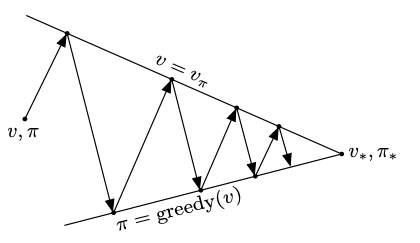
\includegraphics[width=.6\textwidth]{images/GPI2.png}
	\caption{\label{fig:bild2}Iteration between policy evaluation and policy improvement \autocite{Sutton2018}}
	\label{GPI}
\end{figure}

For both policy evaluation and policy improvement different approaches exist. When using \emph{iterative policy evaluation} and a \emph{greedy} policy update, policy iteration is guaranteed to converge to the optimal policy. Iterative policy evaluation describes the evaluation of the current policy using \autoref{valuefunction}. A greedy policy update is selecting the action with the highest expected reward according to a one-step look-ahead using the value function of a consecutive state. 

\chapter{Implementation}

\section{Classes}

\section{Build}

\section{Testing}
\chapter{Extensibility}
% hier weitere Kapitel einbinden

\appendix
% hier Anhänge einbinden
%\input{chapters/sources}

\backmatter

\printbibliography

\clearpage
\thispagestyle{empty}

%Name: \fullname \hfill Matrikelnummer: \matnr \vspace{2cm}
%
%\minisec{Erklärung}
%
%Ich erkläre, dass ich die Arbeit selbständig verfasst und keine anderen als die angegebenen Quellen und Hilfsmittel verwendet habe.\vspace{2cm}
%
%Ulm, den \dotfill
%
%\hspace{10cm} {\footnotesize \fullname}
\end{document}
